\section{Optimization}
\label{sec:eval_optimization}
\begin{itemize}
    \item First part of our evaluation is the optimizations applied by our compiler.
    \item We compare optimizations applied to two different circuits. 
    \item Firstly, classical inputs are provided to the adder,
    \item In the second example, values in superposition will be given to the adder
    \item usual result for classical values, $a = \ket{1}$ $b = \ket{2}$ result in $\ket{3}$
    \item values in superposition result in results in superposition, $a = \ket{3} + \ket{3}$, $b = \ket{2}$ result in $\ket{3}$.
\end{itemize}

\begin{figure}[htp]
    \centering     
    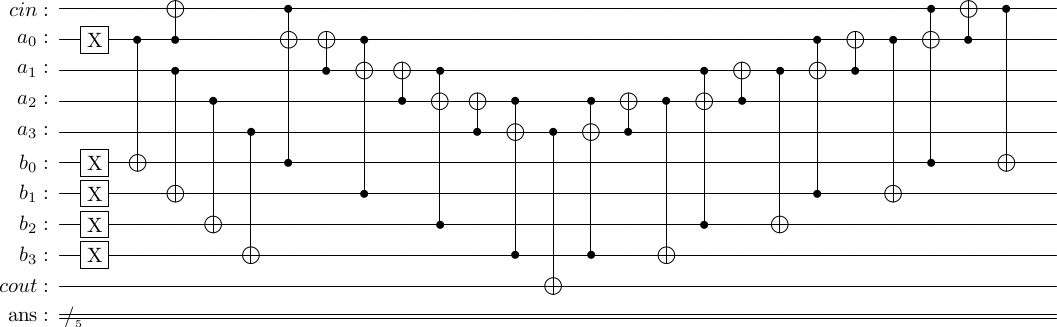
\includegraphics[width=\textwidth]{../figures/images/adderCircuit.png}
    \caption{An unoptimized circuit of a quantum ripple-carry adder.}
    \label{fig:eval_adder_circuit}
\end{figure}

\begin{itemize}
    \item Analyze first and second circuit
    \item How much is optimized?
    \item Depends on input
    \item For only classical, all redundant operations are removed
    \item For input in superposition, optimization effectiveness depends on ``how entangle data''
\end{itemize}


\begin{itemize}
    \item Compare to optimizations performed by quiskit toolkit when transpiling qasm quantum circuit
    \item what is quiskit
    \item what is transpiling
    \item Comparison to quiskit optimizations
    \item What optimizations can be applied
    \begin{itemize}
        \item Which are applied by default optimizations of quiskit of transpilation? -> none
        \item Why? -> no default peeping control rule
        \item Focused on transpilation to a basis gate set and hardware specific optimizations 
        \item In turn, cannot optimize circuit greatly
    \end{itemize}
\end{itemize}


\begin{figure}[htp]
    \centering     
    \lstinputlisting[style=QASM]{../figures/code/evaluation/adder.qasm}
    \caption{An OpenQASM 3 implementation of a quantum ripple-carry adder circuit.}
    \label{fig:eval_adder_qasm}
\end{figure}



\begin{itemize}
    \item (Possibly compiled qasm in appendix)
    \item Quantum Circuit of algorithm  
\end{itemize}


\begin{itemize}
    \item Circuit after optimizations
\end{itemize}